%%%%%%%%%%%%%%%%%%%%%%%%%%%%%%%%%%%%%%%%%%%%%%%%%%%%%%%%%%%
%
% RESULTS
%
%%%%%%%%%%%%%%%%%%%%%%%%%%%%%%%%%%%%%%%%%%%%%%%%%%%%%%%%%%%

\section{Results}

%TODO: Do we add some text here or is this okay?

\subsection{Microsimulation: Non-take-up rates}
%TODO: "Provide graphical visualization (time trend of NTU rates and beta errors) directly within the text for immediate visual impact." - could that be clever @Alex

Our microsimulation results indicate that the non-take-up rate of BAföG, among theoretically eligible students, ranged from approximately 50--70\% across the survey years 2007--2021, with an average of 60\% (Table~\ref{table:microsimulation_ntu}). These estimates are broadly in line with previous findings on non-take-up of social benefits in Germany, which generally fall between around 40--70\%, depending on the program and time period (see Table~\ref{table:NTU-studies} for example). While our estimates are broadly consistent with prior research, they are noticeably higher than the 36--40\% non-take-up rate for BAföG reported by \cite{herber_non-take-up_2019}, who also use SOEP survey data, but for the period 2002--2013.

Several factors may help explain the difference in estimated non-take-up rates. These factors include the specific SOEP variables used to capture income and reported BAföG receipt, as well as differences in the time periods covered (2007 to 2021 in our study versus 2002 to 2013 in \cite{herber_non-take-up_2019}). Other aspects of the microsimulation design and modelling approach may also contribute to the variation. Importantly, the overall accuracy of our model in classifying receipt status is 72\%, as defined by the share of correctly predicted recipients and non-recipients (see equation~\ref{eq:accuracy_microsimulation}). While not perfect, this level of accuracy is consistent with expectations given the complexity of the BAföG system and the limitations of self-reported survey data.

%TODO: can we also say here that this is comparable to some other research that has done this? is that the case? I feel like it might make our case stronger maybe?

%TODO: Also maybe add that the share of all students who take up BAföG has gone down even further since Herbers study (which only covers up to 2013). So in the period between 2013-2021 take up rates declined even further, which presumably also contributes further to our higher average number.

\begin{table}[htbp]
\small
\centering
\begin{tabular}{l@{\hspace{2em}}r@{\hspace{2em}}r@{\hspace{2em}}r}
\toprule
\textbf{Year} & \textbf{Non-Take-Up} & \textbf{Take-Up Rate} & \textbf{Beta Error} \\
              & \(\Pr(\text{NTU} = 1 \mid \text{M} = 1)\) & \(\Pr(\text{TU} = 1 \mid \text{M} = 1)\) & \(\Pr(\text{TU} = 1 \mid \text{M} = 0)\) \\
\midrule
2007 & 60.6 & 39.4 & 13.6 \\
2008 & 63.5 & 36.5 & 17.1 \\
2009 & 61.0 & 39.0 & 18.6 \\
2010 & 60.9 & 39.1 & 17.7 \\
2011 & 53.8 & 46.2 & 16.1 \\
2012 & 51.5 & 48.5 & 18.9 \\
2013 & 50.0 & 50.0 & 15.9 \\
2014 & 55.1 & 44.9 & 16.1 \\
2015 & 64.0 & 36.0 & 12.6 \\
2016 & 56.5 & 43.5 & 12.4 \\
2017 & 62.6 & 37.4 & 10.1 \\
2018 & 63.9 & 36.1 & 15.3 \\
2019 & 67.5 & 32.5 & 11.7 \\
2020 & 63.7 & 36.3 & 13.6 \\
2021 & 66.7 & 33.3 & 12.3 \\
\midrule
\textbf{Average} & \textbf{59.7} & \textbf{40.3} & \textbf{15.0} \\
\bottomrule
\end{tabular}
\caption{\small{Non-Take-Up, Take-Up, and Beta Error Rates by Survey Year (\%). Non-take-up is the share of theoretically eligible students (\(M=1\)) who do not receive BAföG. The take-up rate is simply the complement, i.e., the share of eligible students who do receive BAföG \((1 - \Pr(\text{NTU} = 1 \mid M = 1))\). Beta error is the share of ineligible students (\(M=0\)) who nevertheless receive BAföG.}}
\label{table:microsimulation_ntu}
\end{table}


While there is some variation in non-take-up across years, it remains consistently quite high throughout the period. 
The rate fluctuates from a low of 50\% in 2013 to a high of approximately 68\% in 2019. 
This pattern is clearly illustrated in Figure~\ref{fig:ntu_bounds_over_years}, which shows a visible decline from 2008 up to 2014, followed by a gradual upward trend from 2016 until 2019. 

\begin{figure}[htbp]
  \centering
  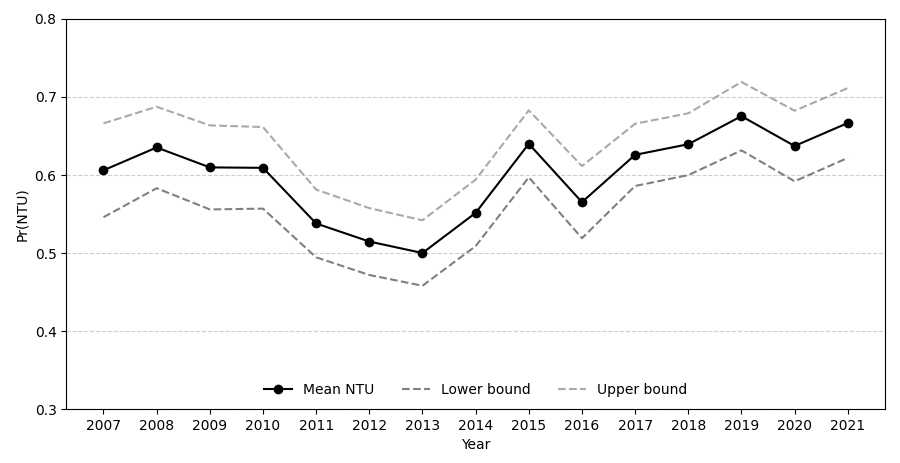
\includegraphics[width=0.95\linewidth]{ntu_bounds.png}
  \caption{Development of the probability of non-take-up from 2007--2021.}
  \label{fig:ntu_bounds_over_years}
\end{figure}

The increase in non-take-up in the years preceding 2021 could potentially reflect behavioural or institutional factors such as changes in awareness, perceived complexity, or attitudes toward debt. 
It could also be partly driven by policy changes. 
Several BAföG reforms were introduced during this period, including increases in grant amounts and adjustments to income thresholds, which may have influenced both eligibility and the perceived attractiveness of the program. 
Since the simulation accounts for these legal changes, the results capture not only behavioural responses, but also how reforms may have affected take-up incentives over time.

%TODO: does this belong in the discussion?

The fourth column in Table~\ref{table:microsimulation_ntu} shows the estimated beta error, which is the share of students who are classified as ineligible by the simulation but report receiving BAföG. 
On average, the beta error is approximately 15\% across the full period. 
This degree of misclassification is similar to what has been observed in other studies of non-take-up, where issues such as income reporting errors and timing mismatches are common \citep{frick_claim_2007}.
While this level of beta error is not negligible, the simulation seems to capture eligibility status fairly well overall, even if some noise is inevitable.

Taken together, the results suggest that a large share of eligible students do not take up BAföG, and that this has been the case fairly consistently over time. 
The high average non-take-up rate, of around 60\%, points to persistent barriers such as lack of information or procedural hurdles. 
The financial attractiveness of BAföG may also be a factor. 
Although support amounts were increased at several points, the need-based allowances have consistently failed to keep pace with the actual cost of living for students \citep{staack_von_2017}. 
This could help explain why some students perceive the benefit as not worth the effort of applying. 
%These findings underline the importance of outreach efforts and suggest that further reforms may be needed to make the program more accessible and appealing.

%TODO: does this also belong in the discussion?

\subsubsection{Stability of Simulated Non-Take-Up under Income Noise}
Table~\ref{tab:conditional_probs_noise_weighted_reduced} reports conditional probabilities of take-up behaviour under varying levels of artificially introduced measurement errors in income. 
To evaluate the robustness of our non-take-up classification, we add normally distributed noise to the log-transformed income variables before recalculating theoretical BAföG entitlements and eligibility indicators. 
The standard deviation of this noise ranges from 0\% (baseline) to 30\%.

\begin{table}[htbp]
\centering
\caption{Conditional probabilities by survey year and noise level}
\begin{tabular}{l|ccc|ccc|ccc|ccc}
\toprule
Year & \multicolumn{3}{c|}{0\%} & \multicolumn{3}{c|}{10\%} & \multicolumn{3}{c|}{20\%} & \multicolumn{3}{c}{30\%} \\
\midrule
2007 & 13.6 & 60.6 & 39.4 & 13.6 & 60.0 & 40.0 & 13.5 & 58.1 & 41.9 & 13.8 & 60.3 & 39.7 \\
2008 & 17.1 & 63.5 & 36.5 & 16.9 & 64.0 & 36.0 & 16.8 & 64.5 & 35.5 & 17.7 & 67.0 & 33.0 \\
2009 & 18.6 & 61.0 & 39.0 & 18.6 & 61.0 & 39.0 & 18.4 & 60.2 & 39.8 & 18.2 & 60.0 & 40.0 \\
2010 & 17.7 & 60.9 & 39.1 & 16.3 & 56.5 & 43.5 & 16.2 & 55.1 & 44.9 & 15.8 & 54.8 & 45.2 \\
2011 & 16.1 & 53.8 & 46.2 & 16.8 & 55.3 & 44.7 & 17.6 & 57.1 & 42.9 & 18.6 & 59.1 & 40.9 \\
2012 & 18.9 & 51.5 & 48.5 & 18.6 & 51.1 & 48.9 & 18.7 & 50.4 & 49.6 & 19.9 & 53.0 & 47.0 \\
2013 & 15.9 & 50.0 & 50.0 & 16.2 & 50.4 & 49.6 & 16.1 & 51.0 & 49.0 & 16.8 & 51.4 & 48.6 \\
2014 & 16.1 & 55.1 & 44.9 & 16.7 & 55.6 & 44.4 & 16.7 & 55.6 & 44.4 & 16.7 & 55.6 & 44.4 \\
2015 & 12.6 & 64.0 & 36.0 & 12.6 & 63.7 & 36.3 & 12.7 & 63.3 & 36.7 & 11.8 & 62.4 & 37.6 \\
2016 & 12.4 & 56.5 & 43.5 & 12.3 & 56.1 & 43.9 & 11.1 & 53.9 & 46.1 & 13.4 & 57.3 & 42.7 \\
2017 & 10.1 & 62.6 & 37.4 & 10.2 & 61.7 & 38.3 & 11.0 & 62.9 & 37.1 & 11.0 & 62.9 & 37.1 \\
2018 & 15.3 & 63.9 & 36.1 & 16.0 & 65.1 & 34.9 & 16.3 & 65.8 & 34.2 & 16.5 & 65.5 & 34.5 \\
2019 & 11.7 & 67.5 & 32.5 & 11.6 & 67.3 & 32.7 & 12.1 & 69.0 & 31.0 & 12.2 & 69.2 & 30.8 \\
2020 & 13.6 & 63.7 & 36.3 & 13.5 & 64.4 & 35.6 & 13.3 & 65.0 & 35.0 & 13.0 & 64.5 & 35.5 \\
2021 & 12.3 & 66.7 & 33.3 & 12.4 & 67.3 & 32.7 & 12.4 & 67.5 & 32.5 & 12.8 & 68.1 & 31.9 \\
\midrule
Total & 15.0 & 59.7 & 40.3 & 15.0 & 59.7 & 40.3 & 15.0 & 59.9 & 40.1 & 15.4 & 60.6 & 39.4 \\
\bottomrule
\end{tabular}
\caption{
 For each noise level (\% std. dev. in log-space). Columns are:
(1) $P(\mathrm{NTU}=0\,|\,M=0)$,
(2) $P(\mathrm{NTU}=1\,|\,M=1)$,
(3) $P(\mathrm{NTU}=0\,|\,M=1)$.
}
\label{tab:conditional_probs_noise}
\end{table}


The findings reveal that simulated take-up probabilities remain highly stable despite income misreporting. 
Across all survey years, the probability of non-take-up changes only slightly, even at the highest noise level. 

This robustness indicates that small to moderate errors in reported income do not significantly impact eligibility classification or population-level take-up estimates. 
It also reflects characteristics of the BAföG eligibility formula, where income thresholds, flat regions, and buffers reduce the sensitivity to minor income fluctuations.

In summary, this analysis reinforces the reliability of our microsimulation approach, demonstrating that the classification of non-take-up is not overly sensitive to realistic levels of income measurement errors.



\subsection{Determinants of Non-take-up: Binary Choice Models}
Table \ref{tab:logit_probit_lpm_results} gives an overview of coefficients and average marginal effects (AME's)\footnote{Where applicable.} of our Logit, Probit and Linear Probability Model.

%TODO: weird footnote

As shown in Table \ref{tab:logit_probit_lpm_results}, all three models consistently indicate that a 100 EUR increase in the simulated BAföG entitlement reduces the probability of non-take-up by approximately two to three percentage points. 
While the Logit and Probit models require average marginal effects for direct probability interpretation due to their nonlinear link functions, the Linear Probability Model coefficients represent approximate percentage point changes directly. 
Differences in magnitude between models are minor and expected given their distinct functional forms.

\begin{table}
\caption*{$\Pr(\mathrm{NTU} = 1 \mid \mathbf{X})$}
\renewcommand{\arraystretch}{1.25}
\centering
\begin{tabular}{lccccc}
\toprule
& \multicolumn{2}{c}{Logit} & \multicolumn{2}{c}{Probit} & LPM \\
& Coef. & AME & Coef. & AME & Coef. \\
\midrule
\multicolumn{6}{l}{\textbf{Main explanatory variables}} \\
Simulated BAföG amount$^{\circ}$ & -0.160*** & -0.029*** & -0.095*** & -0.030*** & -0.021** \\
 & (0.058) & (0.010) & (0.034) & (0.010) & (0.010) \\
\midrule
\multicolumn{6}{l}{\textbf{Controls: Demographics}} \\
Age & 0.099*** & 0.018*** & 0.058*** & 0.018*** & 0.037*** \\
 & (0.019) & (0.003) & (0.011) & (0.003) & (0.003) \\
Female & -0.059 & -0.011 & -0.020 & -0.006 & 0.004 \\
 & (0.256) & (0.047) & (0.149) & (0.046) & (0.046) \\
Has partner & 1.429* & 0.262* & 0.874** & 0.271** & 0.157* \\
 & (0.810) & (0.149) & (0.444) & (0.137) & (0.084) \\
Direct Migration background & -0.700* & -0.128* & -0.419* & -0.130* & -0.130* \\
 & (0.378) & (0.068) & (0.219) & (0.067) & (0.068) \\
Indirect Migration background & -0.689** & -0.127** & -0.407** & -0.126** & -0.121** \\
 & (0.299) & (0.053) & (0.179) & (0.054) & (0.058) \\
\midrule
\multicolumn{6}{l}{\textbf{Controls: Household and Socioeconomic Background}} \\
Living at parents’ home & -0.019 & -0.004 & -0.008 & -0.002 & 0.034 \\
 & (0.270) & (0.049) & (0.160) & (0.050) & (0.048) \\
Sibling claimed BAföG before & -0.554* & -0.102** & -0.321* & -0.100* & -0.107* \\
 & (0.285) & (0.051) & (0.171) & (0.052) & (0.056) \\
East background & -1.253*** & -0.230*** & -0.749*** & -0.232*** & -0.252*** \\
 & (0.313) & (0.052) & (0.186) & (0.054) & (0.061) \\
Parents are highly educated & -0.015 & -0.003 & 0.004 & 0.001 & 0.018 \\
 & (0.293) & (0.054) & (0.175) & (0.054) & (0.052) \\
\midrule
\multicolumn{6}{l}{\textbf{Controls: Behaviour}} \\
Patience & 0.030 & 0.006 & 0.015 & 0.005 & 0.005 \\
 & (0.065) & (0.012) & (0.040) & (0.012) & (0.012) \\
Impulsiveness & -0.039 & -0.007 & -0.021 & -0.006 & -0.009 \\
 & (0.068) & (0.012) & (0.042) & (0.013) & (0.012) \\
Risk Apetite & -0.022 & -0.004 & -0.014 & -0.004 & -0.002 \\
 & (0.037) & (0.007) & (0.021) & (0.007) & (0.006) \\
\midrule
McFadden Pseudo $R^2$ & \multicolumn{2}{l}{0.10} & \multicolumn{2}{l}{0.10} & \\
Likelihood Ratio Test & \multicolumn{2}{l}{53.33 (p = 0.00)} & \multicolumn{2}{l}{53.20 (p = 0.00)} & \\
Adjusted $R^2$ & & & & & 0.74 \\
F-statistic & & & & & 103.8 (p = 0.00) \\
Observations & \multicolumn{5}{l}{458} \\
\bottomrule
\end{tabular}
\caption{Logit, Probit, and LPM (Linear Probability Model) coefficients. Logit and Probit also report average marginal effects. Standard errors are in parentheses. The LPM is estimated via OLS with MacKinnon and White (1985) robust (HC3) standard errors.}
\label{tab:logit_probit_lpm_results}
\caption*{\small{Notes: Significance levels: $^{{*}} p < 0.1$, $^{{**}} p < 0.05$, $^{{***}} p < 0.01$. Robust standard errors clustered at the student level. $\circ$ Indicates per 100 EUR.}}
\end{table}


% Looking at the demographic and socioeconomic predictors, we find that older individuals and those with a registered partner are significantly more likely to forego BAföG despite being eligible. 

The model suggests that age is also a strong predictor of non-take-up in our models: each additional year of age increases the probability of not claiming BAföG by approximately 1.8 percentage points (Logit/Probit AMEs), and 3.7 percentage points in the LPM. 
This positive relationship is consistent with \cite{konijn_quantifying_2023}, who find higher non-take-up with age in the Netherlands. 
In contrast, \cite{herber_non-take-up_2019} report no significant age effect for BAföG in Germany, and \cite{fuchs_austria_2007} find lower non-take-up among older individuals in Austria.\footnote{Fuchs (2007) find a significant negative age effect only in the selection stage of their Heckman model.}
\cite{frick_claim_2007} do not report a consistent or significant effect of age across specifications.

Similarly, the presence of a registered partner corresponds to a substantially higher likelihood of non-take-up, with marginal effects indicating an increase of around 26 (16 in LPM) percentage points. 
These patterns may reflect lower BAföG entitlements among these groups, reducing the perceived benefit of applying. 


Moreover, individuals with direct or indirect migration backgrounds are significantly less likely to refuse BAföG. 
This aligns with \cite{herber_non-take-up_2019} for Germany\footnote{Though not statistically significant.} and \cite{konijn_quantifying_2023} for student aid in the Netherlands. 
By contrast, \cite{fuchs_austria_2007} find no significant effect for social assistance in Austria. 
Similarly, \cite{frick_claim_2007} report mixed results for Germany, with a significant effect only in their Heckman selection model.

Furthermore, all three models suggests that whether an individual lives at home or has moved out from their parents does not, in itself, have a statistically significant effect on the likelihood of BAföG take-up. 
By contrast, informational factors appear to play a more substantial role: having a sibling who has previously received BAföG is associated with a significantly lower probability of non-take-up, by approximately 10 percentage points across all three models. 
This finding highlights the importance of informational spillovers within families in shaping take-up behaviour. 

The models further indicate that individuals with an East German background are significantly more likely to take up BAföG, with non-take-up probabilities reduced by approximately 23 to 25 percentage points across all specifications. 
This finding is consistent with \cite{herber_non-take-up_2019} and \cite{harnisch_nontakeup_2019}, who also report higher take-up rates among individuals from East Germany. 
Detailed descriptive statistics can be found in Appendix~\ref{appendix:tables}, Table~\ref{table:take-up-rates-grouped}.

By contrast, parental education appears to have no meaningful influence on take-up, as the estimated coefficients are statistically insignificant and the AMEs are close to zero across all models, suggesting no substantive effect.

Finally, we do not find any statistically significant effects of the behavioural predictors. 
Specifically, patience, impulsiveness, and self-assessed risk appetite do not have a significant impact on the probability of non-take-up. 
This is in line with \cite{herber_non-take-up_2019}, who also report no significant main effects. 
However, they find statistical significance when interacting impatience and impulsiveness. 
We tested a similar interaction term but found no significant effect. 
Across all models, the estimated coefficients are small and not distinguishable from zero, suggesting that these behavioural traits do not systematically influence BAföG take-up decisions in our sample.


\subsubsection{Restricting to Higher Entitlements}
Our baseline analysis includes all students with any positive simulated BAföG entitlement. 
To check whether our results are driven by those with very small entitlements, who might not consider applying to be worth the effort, we rerun the models restricting the sample to students with simulated monthly entitlements of at least 200 EUR.

As shown in Appendix~\ref{appendix:tables}, Table~\ref{tab:logit_probit_lpm_results_200}, the main findings hold. The negative link between entitlement size and non-take-up remains strong and significant. Similarly, age, partnership status, and East German background continue to show consistent effects. This indicates that the main findings are not just driven by students with minimal entitlements, but also reflect broader patterns in take-up behaviour among those eligible for more substantial benefits.
